
\chapter{Sewer Chamber Design under Critical Conditions using Computational
Fluid Dynamics (CFD)}

This chapter of the dissertation is a manuscript published in Desalination
and Water Treatment, 108 (2018) 1-14, doi: 10.5004/dwt.2018.22019.

Transient sewage flow patterns inside a utility chamber are ... 

\textit{Keywords: }Computational fluid dynamics (CFD); OpenFOAM; Sewer
design; manhole flow; urban runoff

\section{Introduction}

Lorem ipsum dolor sit amet, consectetur adipiscing elit, sed do eiusmod
tempor incididunt ut labore et dolore magna aliqua. Ante metus dictum
at tempor commodo. Quis risus sed vulputate odio ut enim. Sed elementum
tempus egestas sed. Nibh nisl condimentum id venenatis a\citep{Balogh-JoWEaIA-2012-10.1016_j.jweia.2012.02.023,Greifzu-EAoCFM-2016-10.1080_19942060.2015.1104266}.
Et egestas quis ipsum suspendisse ultrices gravida dictum fusce. Tempor
orci eu lobortis elementum nibh tellus molestie nunc. Feugiat pretium
nibh ipsum consequat. Posuere urna nec tincidunt praesent semper feugiat
nibh. Pellentesque dignissim enim sit amet venenatis. Amet purus gravida
quis blandit turpis cursus. Eu ultrices vitae auctor eu augue ut lectus
arcu bibendum. Habitant morbi tristique senectus et. Orci a scelerisque
purus semper eget duis. Elit scelerisque mauris pellentesque pulvinar
pellentesque. Turpis massa sed elementum tempus egestas sed. Eget
mi proin sed libero \citep{Kang-D-2017-10.1016_j.desal.2017.05.018,Kim-DaWT-2017:10.5004_dwt.2017.11423,Kim-DaWT-2017:10.5004_dwt.2017.11422}.
Tempor orci eu lobortis elementum nibh tellus molestie nunc. Feugiat
pretium nibh ipsum consequat. Posuere urna nec tincidunt praesent
semper feugiat nibh. Pellentesque dignissim enim sit amet venenatis.
Amet purus gravida quis blandit turpis cursus. Eu ultrices vitae auctor
eu augue ut lectus arcu bibendum. Habitant morbi tristique senectus
et. Orci a scelerisque purus se  \citep{AhrensGeveciEtAl-2005,Ayachit-2015}.

\section{Simulations}

\subsection{Governing equations}

A brief summary of governing equations is as follows. As noted above,
\texttt{interFoam} is a solver for two incompessible, isothermal,
immiscible fluid, which uses the volume of fluid (VOD) phase fraction.
The continuity and phase-fraction transport equations are 
\begin{equation}
\nabla\cdot\bm{U}=0
\end{equation}
and 
\begin{equation}
\frac{\partial\alpha_{1}}{\partial t}+\nabla\cdot\left(\bm{U}\alpha_{1}\right)=0
\end{equation}
respectively, and the momentum equation is 
\begin{equation}
\frac{\partial\left(\rho\bm{U}\right)}{\partial t}+\nabla\cdot\left(\rho\bm{U}\bm{U}\right)=-\nabla p+\nabla\cdot\bm{T}+\rho\bm{f}_{b}\label{eq:NS}
\end{equation}
where $\alpha_{1}$ is the phase-fraction of water, ranging from 0.0
to 1.0. In Eq. (\ref{eq:NS}), $\bm{T}$ in is the stress tensor and
$\bm{f}_{b}$ is a body force term including gravity and surface tension,
and the fluid density $\rho$ and viscosity $\mu$ are estimated as
\begin{align}
\rho & =\alpha_{1}\rho_{1}+\left(1-\alpha_{1}\right)\rho_{0}\\
\mu & =\alpha_{1}\mu_{1}+\left(1-\alpha_{1}\right)\mu_{0}
\end{align}
where the subscript 1 and 0 indicate water and air phases, respectively.
More details of the solver can be found elsewhere \citep{Weller-CiP-1998-10.1063_1.168744,Manual-OpenFOAMFoundation-2016}.

\subsection{Manhole structure and meshing}

Fig. \ref{fig:manhole-section-view} shows ... 

.

.

This is summarized in Table \ref{tab:dimensions}.

Fig. \ref{fig:mesh-struct} shows .. 

\section{Results and Discussions}

\subsection{Result section title }

Lorem ipsum dolor sit amet, consectetur adipiscing elit, sed do eiusmod
tempor incididunt ut labore et dolore magna aliqua. Morbi tristique
senectus et netus et malesuada. Fusce id velit ut tortor pretium.
Ac turpis egestas integer eget aliquet nibh praesent tristique. Odio
pellentesque diam volutpat commodo sed egestas egestas fringilla.
Maecenas ultricies mi eget mauris. Aliquam purus sit amet luctus.
Amet venenatis urna cursus eget. Turpis tincidunt id aliquet risus.
Eu augue ut lectus arcu bibendum at. Felis imperdiet proin fermentum
leo vel orci porta non. Morbi leo urna molestie at elementum eu. Risus
pretium quam vulputate dignissim suspendisse in est ante in. Nunc
non blandit massa enim. Turpis egestas sed tempus urna. 

\subsection{Tantalizing phenomena}

\subsubsection{3D investigation}

Lorem ipsum dolor sit amet, consectetur adipiscing elit, sed do eiusmod
tempor incididunt ut labore et dolore magna aliqua. Morbi tristique
senectus et netus et malesuada. Fusce id velit ut tortor pretium.
Ac turpis egestas integer eget aliquet nibh praesent tristique. Odio
pellentesque diam volutpat commodo sed egestas egestas fringilla.
Maecenas ultricies mi eget mauris. Aliquam purus sit amet luctus.
Amet venenatis urna cursus eget. Turpis tincidunt id aliquet risus.
Eu augue ut lectus arcu bibendum at. Felis imperdiet proin fermentum
leo vel orci porta non. Morbi leo urna molestie at elementum eu. Risus
pretium quam vulputate dignissim suspendisse in est ante in. Nunc
non blandit massa enim. Turpis egestas sed tempus urna 

\subsubsection{2D investigation}

\subsection{Result verification and convergence test}

In this section, we provide ...

\section{Conclusion}

In order to maintain ...

\paragraph{Acknowledgement}

This research used the Extreme Science and Engineering Discovery Environment
(XSEDE), which is supported by National Science Foundation grant number
ACI-1053575, and was financially supported by R. M. Towill Corporation,
Honolulu, Hawaii, USA. The authors appreciate Mr. Jonathan Imai for
his Solid Works drawing for the mesh generation.

\newpage\null
\vfill
\begin{table}[H]
\begin{centering}
\begin{tabular}{|l|r|r|r|r|}
\hline 
 & $D$ & $L$ & $W$ & $H$\tabularnewline
\hline 
\hline 
inlet pipe & 16.0 in. (0.406 m) & 16.0 ft (4.9 m) & -- & --\tabularnewline
\hline 
outlet pipe & 18.0 in. (0.457 m) & 22.0 ft (6.7 m) & -- & --\tabularnewline
\hline 
chamber & -- & 10.0 ft (3.0 m) & 4.0 ft (1.2 m) & 6.0 ft (1.8 m)\tabularnewline
\hline 
\end{tabular}
\par\end{centering}
\caption{Chamber and pipe dimensions. CFD simulations were conducted for three
outlet diameters: 18, 20, and 24 inches (0.457, 0.508, and 0.610 meters,
respectively).}

\label{tab:dimensions}
\end{table}

\vfill\newpage\null
\vfill
\begin{table}[H]
\begin{centering}
\begin{tabular}{|l|c|c|c|}
\hline 
 & water & air & unit\tabularnewline
\hline 
\hline 
fluid type & Newtonian & Newtonian & -\tabularnewline
\hline 
density, $\rho$ & 998.0 & 1.21 & kg/m\textsuperscript{3}\tabularnewline
\hline 
kinematic viscosity, $\nu$ & $1.0\times10^{-6}$ & $1.51\times10^{-5}$ & m\textsuperscript{2}/s\tabularnewline
\hline 
\end{tabular}
\par\end{centering}
\caption{Properties of water and air used for \texttt{interFoam} simulations.
In addition, the surface tension between water and air was set as
0.072 N/m and the gravitational acceleration (9.81m/s\protect\protect\textsuperscript{2})
was used.}

\label{tab:matt-prop}
\end{table}

\vfill\newpage\null
\vfill
\begin{figure}[H]
\begin{centering}
\includegraphics[width=5in]{Figures/Fig01-manhole-simple}
\par\end{centering}
\caption{Section view of a real manhole.}
\label{fig:manhole-section-view}
\end{figure}

\vfill

\newpage\null
\vfill
\begin{figure}[H]
\begin{centering}
(a)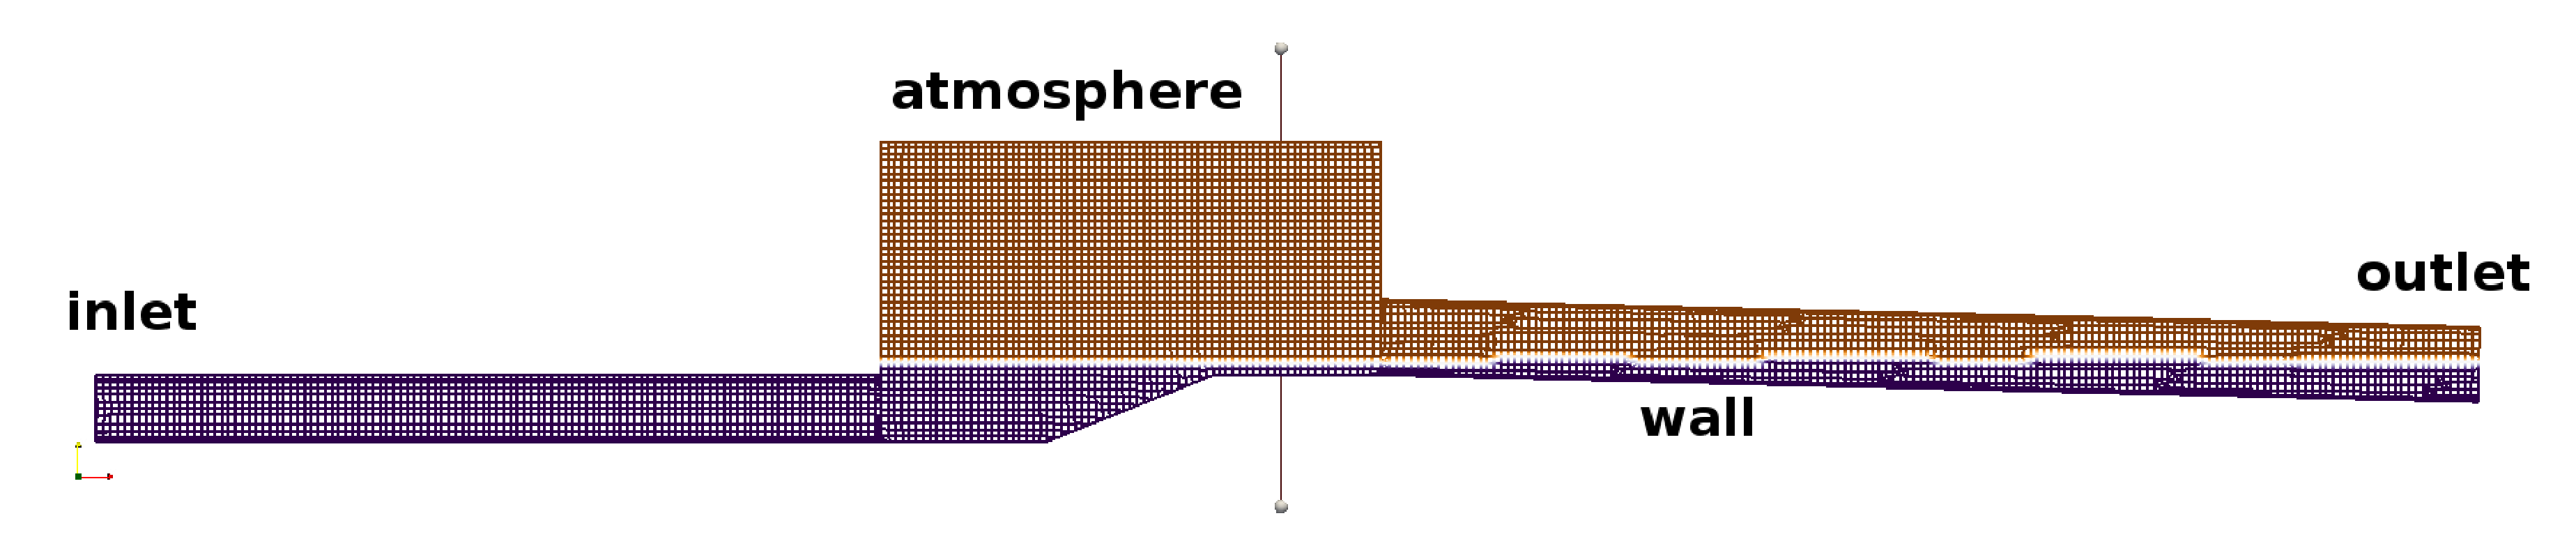
\includegraphics[width=6in]{Figures/Fig02-Mesh-2D-antd}
\par\end{centering}
\begin{centering}
(b)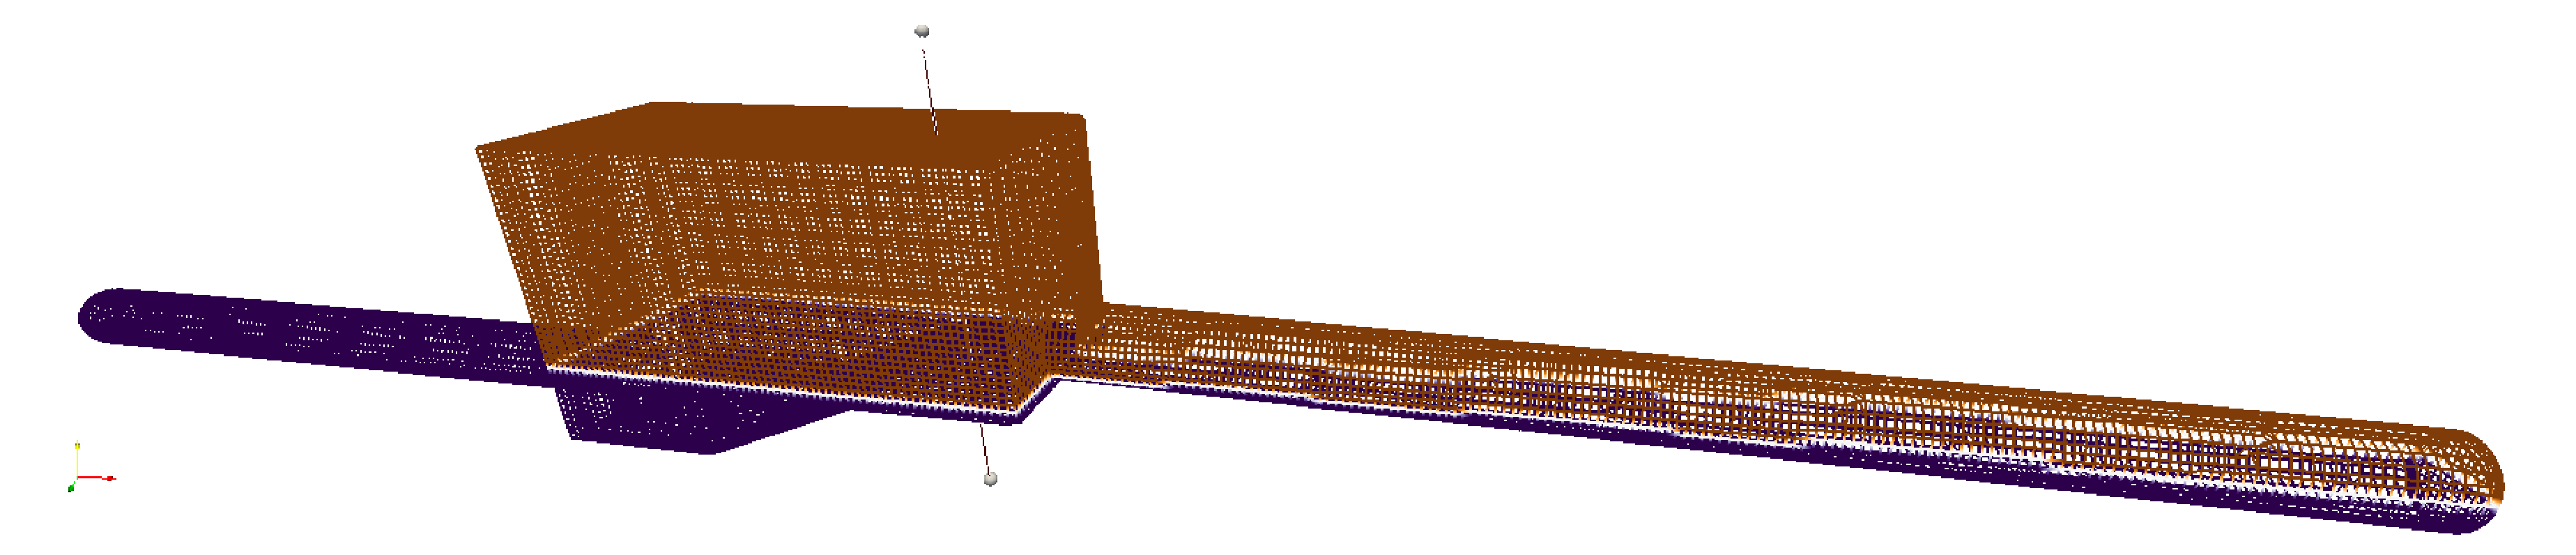
\includegraphics[width=6in]{Figures/Fig02-Mesh-3D}
\par\end{centering}
\caption{Generated mesh structures: (a) 2D and (b) 3D views. The lower purple
and upper brown regions represent water and air phases, respectively.
The vertical line in the $y$-direction near the chamber outlet indicates
a line through which sewage levels are calculated using OpenFOAM simulation
results. In addition, $x$-direction is along the left inlet pipe,
and $z$-direction is out of the $x-y$ plane.}

\label{fig:mesh-struct}
\end{figure}

\vfill
